\chapter{Automatic Lesion VOI Delineation}
\label{app:lesion_voi_delineation}

This appendix documents the automatic lesion-mask construction used to define
fixed inputs for the patient analysis in Chapter~\ref{chapter:paper}. The
procedure was adapted from the gradient-based PET segmentation method of
Mikell \textit{et al.} \cite{mikellImpact90YPET2018}, with pragmatic bounds
added for the present post-\glsentryshort{sirt} data. It was not evaluated as
a separate methodological contribution, and no delineation-accuracy or
parameter-sensitivity study was performed.

\section{Candidate selection}

For each patient, candidate seed voxels were identified on the vendor Q.Clear
$\beta$-4000 \glsentryshort{pet} reconstruction and ordered from highest to
lowest intensity. Seeds were required to be separated by at least
\SI{30}{\milli\metre}. Candidate masks were grown in this order, and masks
containing fewer than 10 voxels were discarded. The five highest-ranked
non-overlapping masks were retained. If two candidates overlapped, the mask
grown from the hotter seed was retained and the lower-ranked candidate was
discarded.

\section{Radial-gradient growth}

The vendor image was smoothed with a Gaussian kernel ($\sigma=0.1$). Rays were
cast outwards from each seed, and the candidate boundary in each direction was
located from the maximum image-gradient magnitude within the admissible search
interval. Figure~\ref{fig:lesion_grower_radial} illustrates the seed-centred
radial search and the corresponding gradient-magnitude image.

\begin{figure}[htbp]
    \centering
    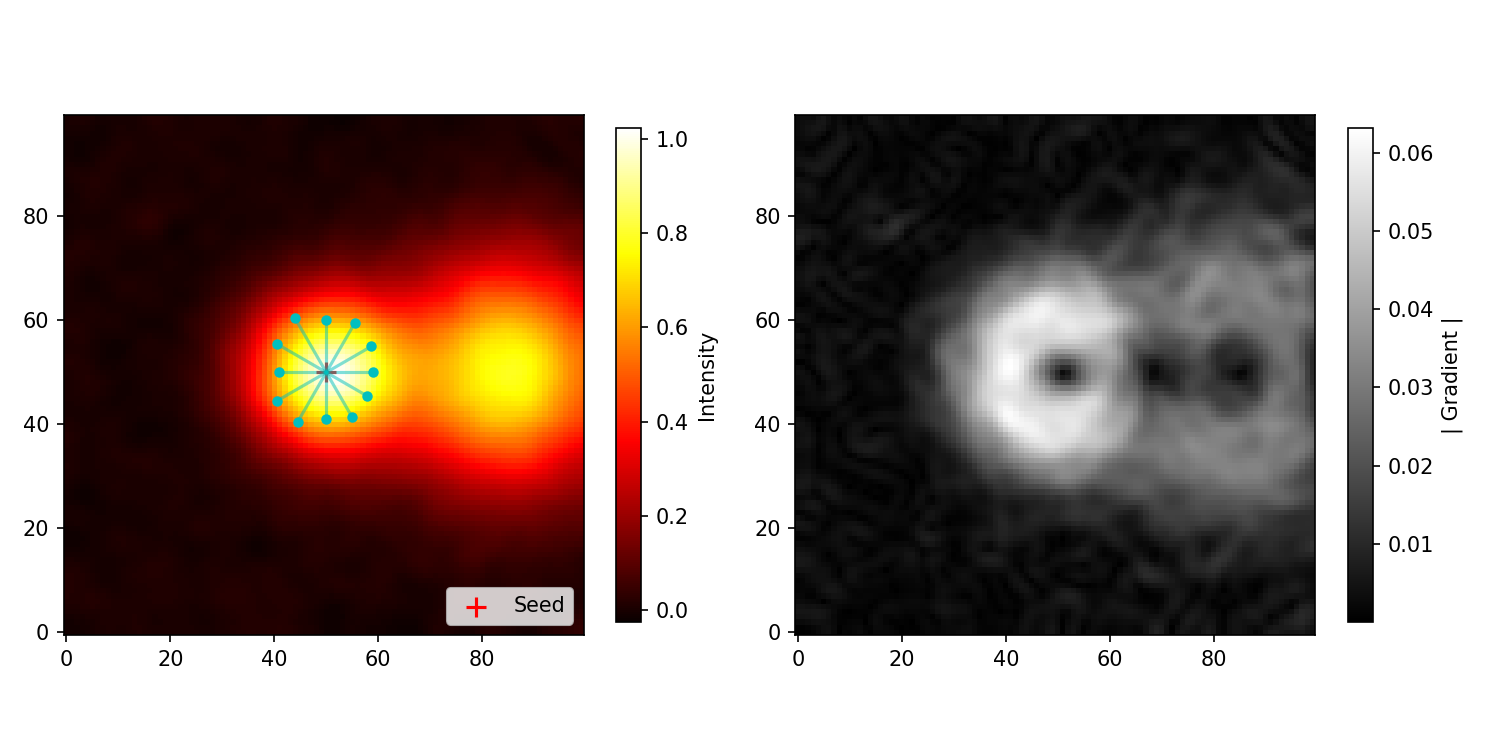
\includegraphics[width=0.95\linewidth]{figures/lesion_grower/lesion_grower_2d_visualization.png}
    \caption{Two-dimensional illustration of radial-gradient lesion
    delineation. Left: radial searches extend from the seed voxel to candidate
    boundary locations. Right: the corresponding image-gradient magnitude
    used to identify the lesion edge. This schematic illustrates the search
    principle; patient masks were generated in the image volume.}
    \label{fig:lesion_grower_radial}
\end{figure}

Two safeguards bounded each radial search. First, the maximum ray length was
\SI{25}{\milli\metre}, preventing a ray from reaching a spatially separate
hot lesion. Second, samples were restricted to intensities above the
background-adjusted floor
\begin{equation}
I_{\mathrm{floor}}
=I_{\mathrm{bkg}}+0.42\left(I_{\mathrm{seed}}-I_{\mathrm{bkg}}\right),
\label{eq:lesion_growth_floor}
\end{equation}
where $I_{\mathrm{bkg}}$ is the mean intensity in the patient-specific liver
background \glsentryshort{voi}. The floor therefore retains 42\% of the
contrast between the seed and the background. This fraction lies within the
36--44\% range reported by Erdi \textit{et al.} for PET lung-lesion
delineation \cite{erdiSegmentationLungLesion1997}. For those data the
background was comparatively low; here, the non-zero liver background was
retained explicitly. Because the published thresholds depended on imaging
conditions and were not derived for post-\glsentryshort{sirt} $^{90}$Y liver
lesions, Equation~\eqref{eq:lesion_growth_floor} was used as a pragmatic
stopping bound rather than as a separately validated threshold.

\begin{figure}[htbp]
    \centering
    \begin{subfigure}[t]{0.98\linewidth}
        \centering
        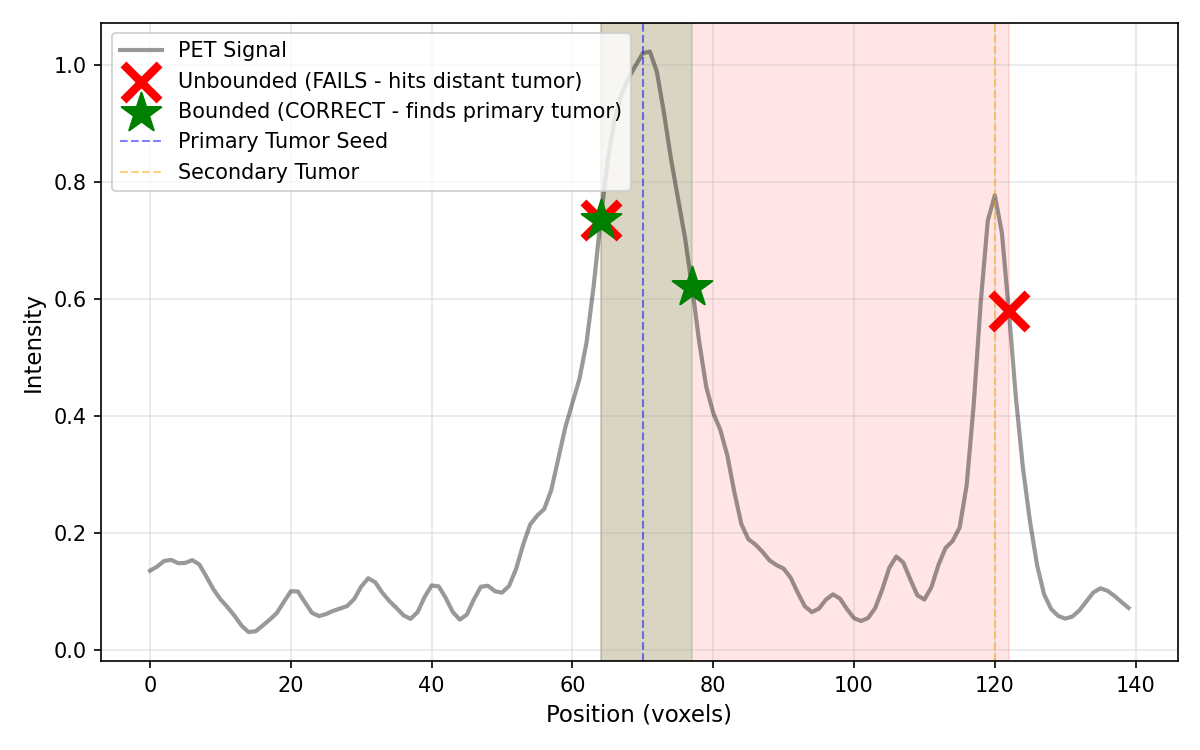
\includegraphics[width=0.85\linewidth]{figures/lesion_grower/demo1_bounded_spokes.png}
        \caption{Maximum-distance bound. Without a bounded search, a ray can
        encounter the gradient associated with a separate hot lesion.}
    \end{subfigure}

    \medskip

    \begin{subfigure}[t]{0.98\linewidth}
        \centering
        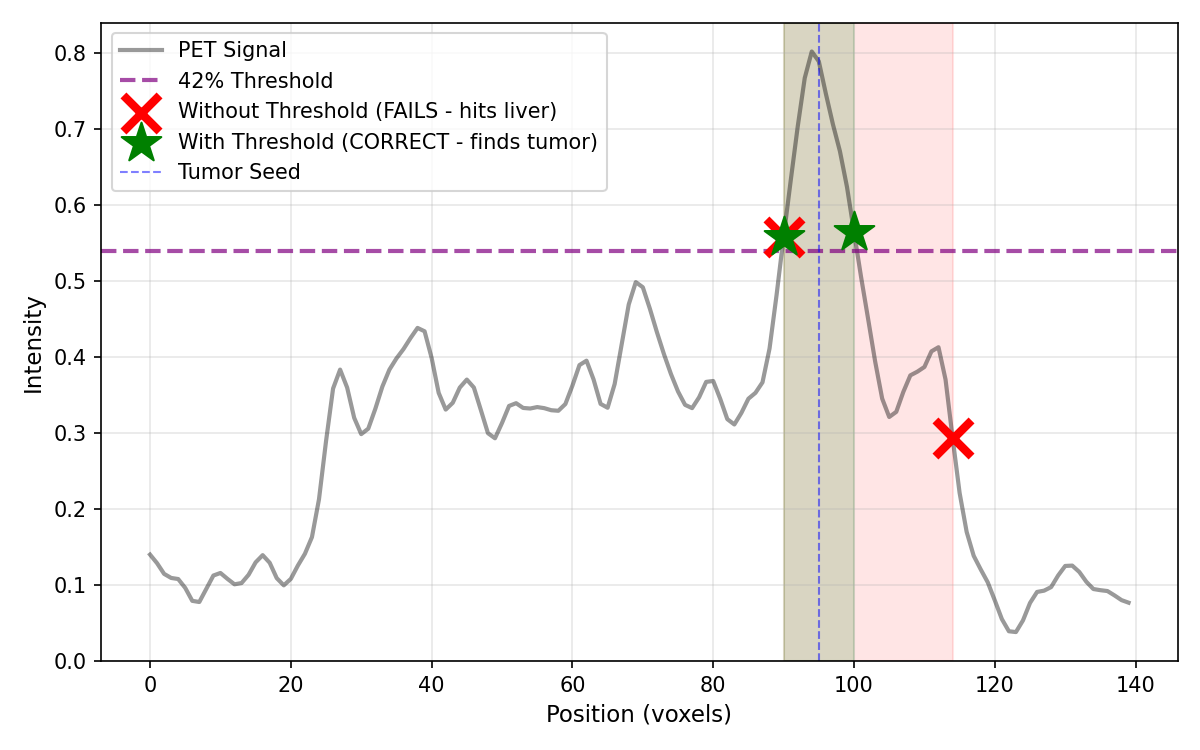
\includegraphics[width=0.85\linewidth]{figures/lesion_grower/demo2_intensity_threshold.png}
        \caption{Background-adjusted intensity bound. Restricting the
        admissible search interval prevents a gradient in the surrounding
        liver background from being selected as the lesion boundary.}
    \end{subfigure}
    \caption{Illustrative safeguards used to bound the radial-gradient search.
    The curves are schematic one-dimensional profiles rather than patient
    measurements.}
    \label{fig:lesion_grower_bounds}
\end{figure}
